\documentclass[notes,10pt]{beamer}
\usetheme[
%%% option passed to the outer theme
%    progressstyle=fixedCircCnt,   % fixedCircCnt, movingCircCnt (moving is deault)
  ]{Feather}
  
% If you want to change the colors of the various elements in the theme, edit and uncomment the following lines

% Change the bar colors:
%\setbeamercolor{Feather}{fg=red!20,bg=red}

% Change the color of the structural elements:
%\setbeamercolor{structure}{fg=red}

% Change the frame title text color:
%\setbeamercolor{frametitle}{fg=blue}

% Change the normal text color background:
%\setbeamercolor{normal text}{fg=black,bg=gray!10}

%-------------------------------------------------------
% INCLUDE PACKAGES
%-------------------------------------------------------

\usepackage[utf8]{inputenc}
\usepackage[ngerman]{babel}
\usepackage[T1]{fontenc}
\usepackage{helvet}
\usepackage{eurosym}

%-------------------------------------------------------
% DEFFINING AND REDEFINING COMMANDS
%-------------------------------------------------------

% colored hyperlinks
\newcommand{\chref}[2]{
  \href{#1}{{\usebeamercolor[bg]{Feather}#2}}
}

%-------------------------------------------------------
% INFORMATION IN THE TITLE PAGE
%-------------------------------------------------------

\title[] % [] is optional - is placed on the bottom of the sidebar on every slide
{ % is placed on the title page
      \textbf{Ransomware}
}

\subtitle[Ransomware]{}

\author[S. Abwandner, M. Beham, P. Schmid]
{      Sebastian Abwandner, Michael Beham, Pascal Schmid 
}

\institute[]
{
      Hochschule Augsburg  \\
      University of Applied Sciences Augsburg
}

\date{\today}

%-------------------------------------------------------
% THE BODY OF THE PRESENTATION
%-------------------------------------------------------

\begin{document}

%-------------------------------------------------------
% THE TITLEPAGE
%-------------------------------------------------------

{\1% % this is the name of the PDF file for the background
\begin{frame}[plain,noframenumbering] % the plain option removes the header from the title page, noframenumbering removes the numbering of this frame only
  \titlepage % call the title page information from above
\end{frame}}


\begin{frame}{Gliederung}{}
\tableofcontents
\end{frame}

%-------------------------------------------------------
\section{Kleine Viren-Kunde}
%-------------------------------------------------------
\begin{frame}{Kleine Viren-Kunde}
%-------------------------------------------------------
	\begin{figure}[p]
		\centering
		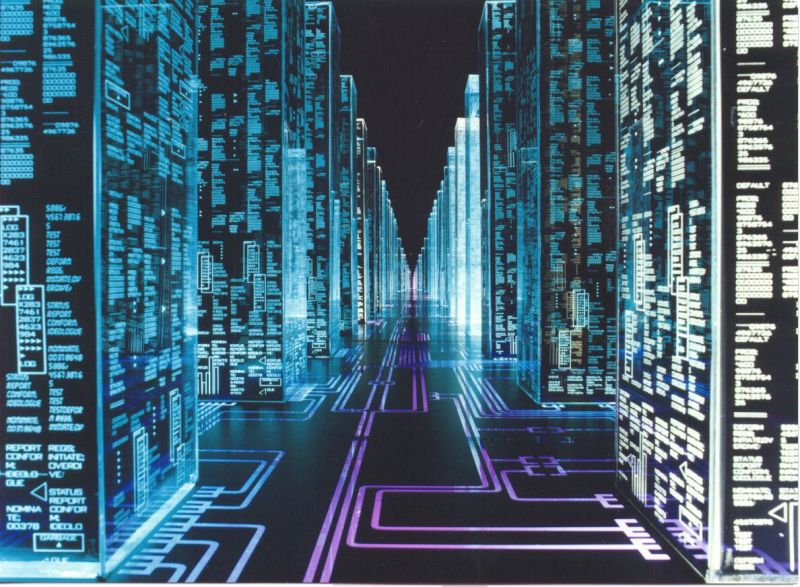
\includegraphics[scale=0.3]{hackers_internet.jpg}
		\let\thefootnote\relax\footnote{https://hackadaycom.files.wordpress.com/2013/03/hackers\_internet.jpg}
	\end{figure} 
\end{frame}

\begin{frame}{Kleine Viren-Kunde}{Wer verwendet Viren?}
%-------------------------------------------------------
\begin{itemize}
	\item Security Researcher
	\item Anonymous
	\item Extremisten
	\item Regierungen (Bundestrojaner, Stuxnet)
	\item Sonstige Kriminelle
	\item Scriptkiddies
\end{itemize}
\end{frame}

\begin{frame}{Kleine Viren-Kunde}{Arten von Viren}
%-------------------------------------------------------
\begin{itemize}
	\item Viren, Würmer, Trojaner
	\item Botnetze
	\item Ransomware
\end{itemize}
\end{frame}

\begin{frame}{Kleine Viren-Kunde}{DOS-Viren}
%-------------------------------------------------------
	\begin{figure}[p]
		\centering
		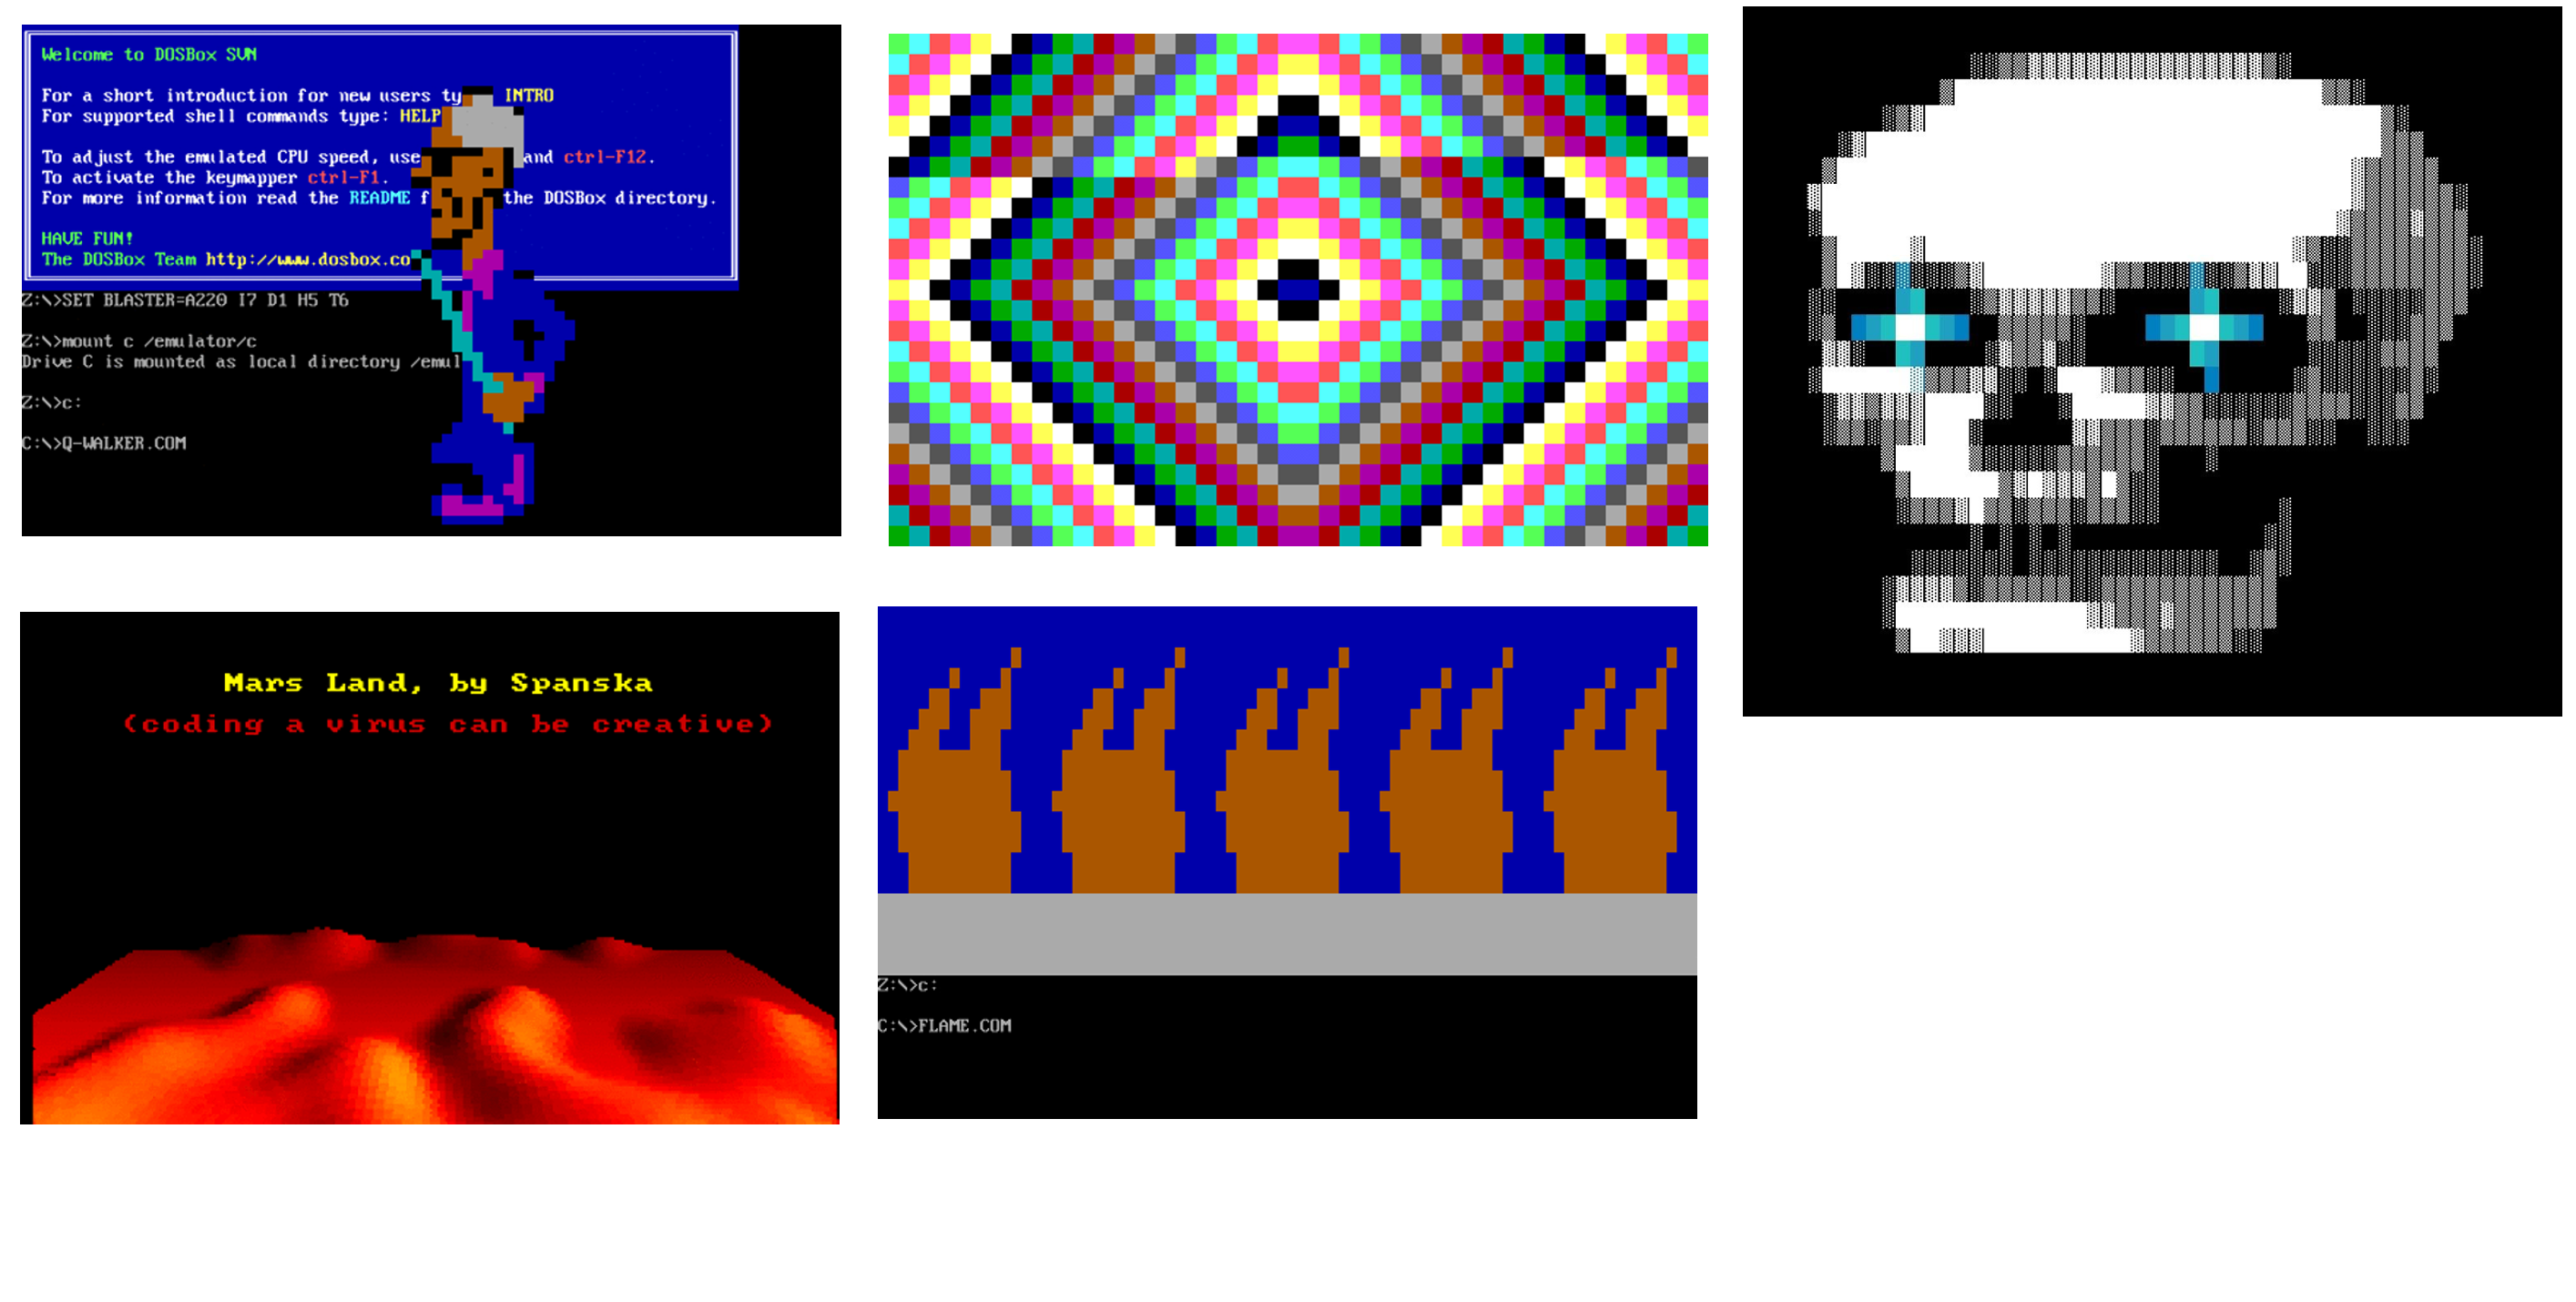
\includegraphics[scale=0.11]{dos_viruses.png}
		\let\thefootnote\relax\footnote{\url{https://archive.org/details/malwaremuseum}}
	\end{figure}
\end{frame}


\begin{frame}{Kleine Viren-Kunde}{Botnetze}
%-------------------------------------------------------
	\begin{itemize}
		\item Massenhaft übernommene Computer
		\item Alle Platformen
		\item Kapazität wird vom Botnetz-Betreiber vermietet
	\end{itemize}
\end{frame}


\begin{frame}{Kleine Viren-Kunde}{Ransomware Unterscheidung}
%-------------------------------------------------------

	\begin{figure}[p]
		\centering
		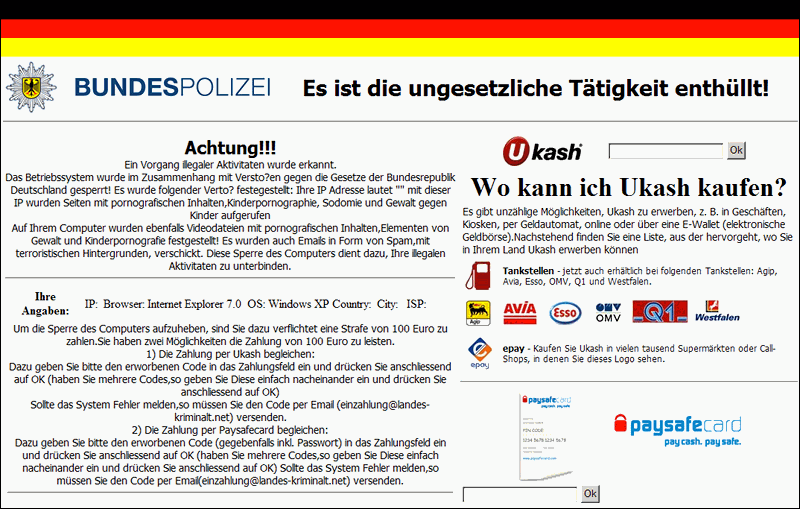
\includegraphics[scale=0.25]{bka-trojaner.png}
		\let\thefootnote\relax\footnote{\url{http://bka-trojaner.de/screenshots/bka-trojaner2.png}}
	\end{figure}

\end{frame}

\begin{frame}{Kleine Viren-Kunde}{Ransomware Unterscheidung}
%-------------------------------------------------------

	\begin{block}{Locker Ransomware}
		\begin{itemize}
			\item FBI, BKA, Bundespolizei, ...
			\item Entfernen leicht möglich, da kein Schaden
			\item Was bringt Zukunft?
			\note{Bei IoT z.B. ist Interaktion nicht/kaum möglich\\}
	   	\end{itemize}
	   	\note{Locker Ransomware war nur für Heimanwender brauchbar. Admins wussten sich dagegen zu wehren}
	\end{block}
 	\begin{block}{Crypto Ransomware}
	  	\begin{itemize}
			\item Nutzer hat Schaden
			\item Entfernen schwierig
	   	\end{itemize}
  	\end{block}

\end{frame}

\begin{frame}{Kleine Viren-Kunde}{AIDS}
%-------------------------------------------------------
	\begin{figure}[p]
		\begin{itemize}
			\item Trojaner \textbf{AIDS} (1989)
			\item Infektion über präparierte Diskette
			\item Nach dem 90. Boot: \\ Verschlüsselung aller Daten auf der Systemfestplatte
			\item Aufforderung ca. \EUR{170} an ein Postfach in Panama zu senden
		\end{itemize}
		\let\thefootnote\relax\footnote{c't Magazin 07/2016 S.77}
	\end{figure}
\end{frame}

\begin{frame}{Kleine Viren-Kunde}{Geschichte der Ransomware}
%-------------------------------------------------------
	\begin{itemize}
		\item<1-> 1989: AIDS
		\item<2-> 2013: CryptoLocker (Windows)
		\note[item]<2>{\textbf{Cryptolocker:}}
		\note[item]<2>{(40\% aller Betroffenen zahlten}
		\note[item]<2>{insgesamt ca. 3 Millionen \$}
		\note[item]<2>{scannt Netzlaufwerke und angeschlossene USB-Geräte, ...)}
		\item<3-> 2013: FBI ransomware (OS X)
		\item<4-> 2014: Simplocker (Android)
		\item<4-> 2014: Oleg Pliss (iOS) (Locker Ransomware)
		\item<5-> 2016: Locky (Windows)
		\item<5-> 2016: KeRanger (OS X)
	\end{itemize}
\end{frame}

\begin{frame}{Kleine Viren-Kunde}{Evolution der Ransomware}
%-------------------------------------------------------
	\begin{figure}[p]
		\centering
		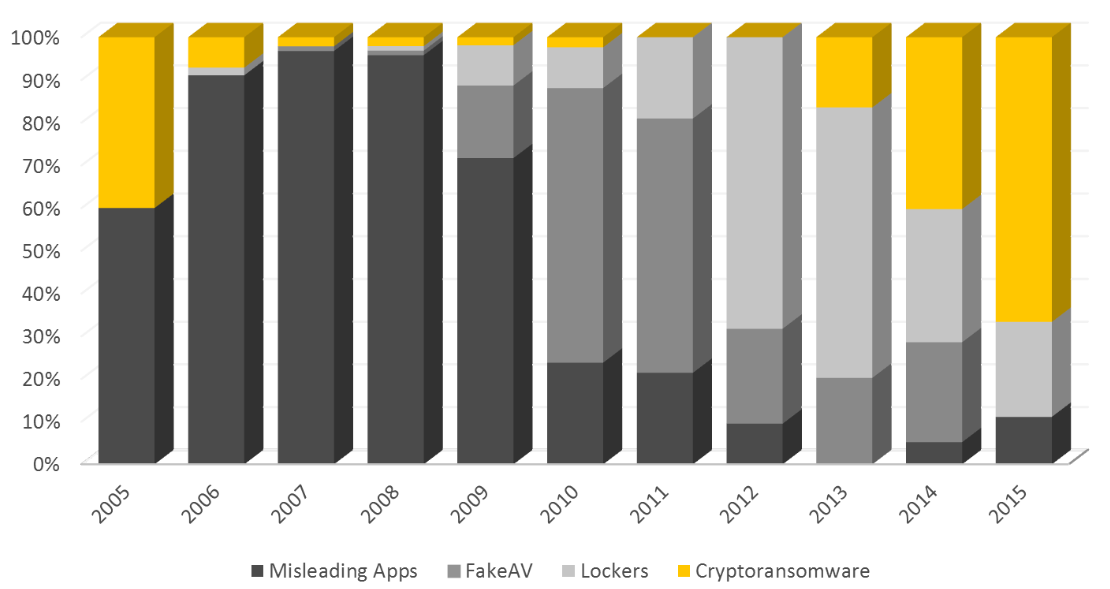
\includegraphics[scale=0.28]{ransom-evolution.png}
		\let\thefootnote\relax\footnote{\url{https://www.symantec.com/content/en/us/enterprise/media/security\_response/whitepapers/the-evolution-of-ransomware.pdf}}
		\note{Wegen schlechter anonymer internationaler Zahlungsmöglichkeit ist Anzahl von Ransomware bis zum Erscheinen von Bitcoin zurück gegangen}
	\end{figure}
\end{frame}


%-------------------------------------------------------
\section{Ransomware}
%-------------------------------------------------------
\subsection{Aktuelle Beispiele}
\begin{frame}{Dettelbach}
%-------------------------------------------------------

	\begin{itemize}
		\item Stadtverwaltung von Dettelbach (Unterfranken)
		\item Server mit "`Tesla-Crypt"' infiziert
		\item Infektion wahrscheinlich per E-Mail-Anhang
		\item Backups vorhanden\pause , aber nicht wiederherstellbar
		\item Nach Zahlung von ca. \EUR{490} konnten große Teile der Daten entschlüsselt werden
	\end{itemize}
	\let\thefootnote\relax\footnote{\url{https://www.polizei.bayern.de/unterfranken/news/presse/aktuell/index.html/237562}}
\end{frame}

\begin{frame}{Lukaskrankenhaus Neuss}
%-------------------------------------------------------

	\begin{itemize}
		\item Infektion ebenfalls per E-Mail-Anhang
		\item Sofortmaßnahme: Abschalten aller Dienste und Server (intern und extern) \pause
		\item Organisation mit Formularen auf Papier (Notfallplan vorhanden)
		\item Aktuelles Backup vorhanden\pause , und auch wiederherstellbar
	\end{itemize}
	\let\thefootnote\relax\footnote{\url{http://www1.wdr.de/cyberangriff-lukaskrankenhaus-neuss-100.html}}
\end{frame}

\section{Kryptographie}
\subsection{Symmetrische Verschlüsselung}
\begin{frame}{Symmetrische Verschlüsselung}
	\begin{itemize}
		\item Gleicher Schlüssel für Ver- und Entschlüsselung
		\item Typischer Vertreter: \textbf{AES} (Advanced Encryption Standard)
		\item Schneller Algorithmus mit Prozessorunterstützung
		\item Geeignet auch für große Datenmengen
	\end{itemize}
\end{frame}
\subsection{Asymmetrische Verschlüsselung}
\begin{frame}{Asymmetrische Verschlüsselung}
	\begin{itemize}
		\item Zwei Schlüssel: Verschlüsselung und Entschlüsselung (Öffentlich / Privat)
		\item Mathematisch sicher bei großer Schlüssellänge (4096 Bit)
		\item Großer Rechenaufwand, daher nicht für große Datenmenge geeignet
	\end{itemize}
\end{frame}
\subsection{Hybride Verschlüsselung}
\begin{frame}{Hybride Verschlüsselung}
	\begin{itemize}
		\item Sitzungsschlüssel zufällig erzeugen
		\item Sitzungsschlüssel für AES verwenden
		\item Sitzungsschlüssel asymmetrisch verschlüsseln
	\end{itemize}
\end{frame}

\section{Ransomware}
\subsection{Beispiele}
\begin{frame}{Ransomware}{Beispiele}
	\begin{itemize}
		\item Encryptor RaaS (Ransomware as a Service)
		\item TeslaCrypt (Version 2.0, 3.0, 4.0)
		\item Locky
		\item CryptoLocker
		\item Cryptowall
	\end{itemize}
\end{frame}

\subsection{Funktionsweise}
\begin{frame}{Ransomware}{Infektion}
		\begin{itemize}
			\item weite Streuung
			\item meist unspezifisch
			\item Verbreitungswege:
				\begin{itemize}
					\item E-Mail
					\item Webseiten (Drive-By-Downloads, Wordpress)
					\item Makros (Excel, Word)
				\end{itemize}
			\item Umgehen der Heuristiken von Virenscannern (Warten)
		\end{itemize}
\end{frame}
\begin{frame}{Ransomware}{Angriff}
		\begin{itemize}
			\item C\&C-Server finden und kontaktieren 
			\item Asym. Schlüssel erstellen (Öffentlich und Privat)
			\item Privaten Schlüssel an Server senden und lokal vernichten
			\item Dateien verschlüsseln:
				\begin{itemize}
					\item Zufälligen Sitzungsschlüssel erstellen
					\item Datei damit verschlüsseln
					\item Sitzungsschlüssel mit öffentlichen Schlüssel verschlüsseln und mit Datei speichern
					\item Sitzungsschlüssel vernichten
				\end{itemize}
			\item Nutzer informieren
		\end{itemize}
\end{frame}


%-------------------------------------------------------
\subsection{Required Packages}
\begin{frame}{Installation}{Required Packages}
%-------------------------------------------------------

  For using the Feather Theme you will need the Bemaer class installed and the following 2 packages
  \begin{itemize}
    \item TikZ\footnote{TikZ is a package for creating beautiful graphics. Have a look at these \chref{http://www.texample.net/tikz/examples/}{online examples} or the \chref{http://tug.ctan.org/tex-archive/graphics/pgf/base/doc/generic/pgf/pgfmanual.pdf}{pgf user manual}.}
    \item calc
  \end{itemize}
  Due to the fact that the packages are very common they should be included in your latex distribution in the first place.
\end{frame}

%-------------------------------------------------------
\section{User Interface}
\subsection{Loading the Theme and Theme Options}
\begin{frame}{User Interface}{Loading the Theme and Theme Options}
%-------------------------------------------------------

  \begin{block}{The Presentation Theme}
    The Feather Theme can be loaded in a familiar way. In the reamble of your {\tt tex} file you must type\\ \vspace{5pt} 
    {\tt \textbackslash usetheme[<options>]\{Feather\}}\\ \vspace{5pt} 
    The presentation theme loads the inner, outer and color Feather theme files and passes the {\tt <options>} on to these files.
  \end{block}
  \begin{block}{The Inner and Outher Themes}
    If you wish you can load only the inner, or the outher theme directly by\\ \vspace{5pt} 
    {\tt \textbackslash useinnertheme\{Feather\}} (and it has no options)\\ \vspace{5pt} 
    {\tt \textbackslash useoutertheme[<options>]\{Feather\}} (it has one option)\\
    \hspace{20pt}{\tt progressstyle=\{fixedCircCnt or movingCircCnt\}} \\
    \begin{itemize}
    \item which set how the progress is illustrated;
    \item the value {\tt movingCircCnt} is the default.
    \end{itemize}
  \end{block}
\end{frame}

\begin{frame}{User Interface}{Loading the Theme and Theme Options}

  \begin{block}{The Color Theme}
    Also you can load only the color theme by writing in the preamble of the {\tt tex} file 
    
    \vspace{5pt} 
    
    \begin{itemize}
    \item {\tt \textbackslash usecolortheme\{Feather\}}
    \end{itemize}
    
    \vspace{5pt}
    
    ...or to change the colors of the various elements in the theme
    
    \vspace{5pt} 
    \begin{itemize}
    \item Change the bar colors: \\    
    {\tt \textbackslash setbeamercolor \{Feather\}\{fg=<color>, bg=<color>\}}
    
    \vspace{2pt} 
    
    \item Change the color of the structural elements: \\    
    {\tt \textbackslash setbeamercolor\{structure\}\{fg=<color>\}}
    
    \vspace{2pt} 
    
    \item Change the frame title text color:\\
    {\tt \textbackslash setbeamercolor\{frametitle\}\{fg=<color>\}}
    
    \vspace{2pt} 
    
    \item Change the normal text color background:    
    {\tt \textbackslash setbeamercolor\{normal text\}\{fg=<color>, bg=<color>\}}
    \end{itemize}
  \end{block}
\end{frame}


%-------------------------------------------------------
\subsection{Feather image}
\begin{frame}{User Interface}{The Feather Background Image}
%-------------------------------------------------------

\begin{block}{The Feather Background Image}
    \begin{itemize}
    \item In Feather theme, the title page frame and the last frame have the Feather image as the background image. 
    \item The Feather background image can be produced to any frame by wrating on the begining at the choosen frame the following
    \end{itemize} 
    
    \vspace{5pt} 
    
  {\tt \{\textbackslash 1bg\\
    \textbackslash begin\{frame\}[<options>]\{Frame Title\}\{Frame Subtitle\}\\
    \ldots\\
    \textbackslash end\{frame\}\}}
\end{block}
\end{frame}



{\1
\begin{frame}[plain,noframenumbering]
  \finalpage{Vielen Dank für Eure Aufmerksamkeit!}
\end{frame}}

{\1
\begin{frame}[plain,noframenumbering]
	\begin{figure}[p]
		\centering
		
\includegraphics[scale=0.1]{questionmark.png}
	\end{figure}  
\end{frame}}

\end{document}